\documentclass{beamer}
\usepackage[utf8]{inputenc}
\usepackage{amsthm}
\usepackage{amsmath}
\usepackage{graphicx}
\usetheme{Madrid}
\title{Control Systems (EE2227)}
\author{Abhishek}
\institute{IIT Hyderabad}

\begin{document}
\frame{\titlepage}
\begin{frame}{Question}
Consider the following second order system with the transfer function:
$$G(s) = \frac{1}{1+2s+s^2}$$
\\with input unit step $$R(s) = \frac{1}{s}$$  Let C(s) be the corresponding output. The time taken by the system output c(t) to reach 94\% of its steady state value, rounded off to two decimal places is
\medskip
\\ \hspace{20}(A)5.25\hspace{20}(B)4.50 \hspace{20}(C)3.89  \hspace{20}(D)2.81


\end{frame}
\begin{frame}{Answer}
The approach for finding the solution is as follows:
\begin{itemize}
    \item finding C(s)
    \item finding c(t)
    \item finding the time at which c(t) attains 94\% of its steady state value
\end{itemize}
\end{frame}
\begin{frame}{Finding C(s)}
We are given G(s) and R(s), to find C(s), we can simply multiply these two
$$C(s) = R(s).G(s) = (\frac{1}{s})  (\frac{1}{1+2s+s^2})$$
$$C(s) =  \frac{1}{s(1+s)^2}
\end{frame}
\begin{frame}{Finding c(t)}
To find c(t), we have to do inverse Laplace transform on C(s)
$$c(t) \longleftrightarrow C(s)$$
Inverse Laplace transform can be calculated by the formula:
$$f(t) = \frac{1}{2\pi j} \int_{a -j\infty}^{a+j\infty}F(s)e^{st} ds$$
From the above formula, the inverse Laplace for some common expressions are:
$$u(t) \longleftrightarrow \frac{1}{s}$$
$$e^{-at} u(t) \longleftrightarrow \frac{1}{s+a}$$
$$t e^{-at} u(t) \longleftrightarrow \frac{1}{(s+a)^2}$$
    
\end{frame}
\begin{frame}{Finding c(t)}
We found C(s) as:
$$C(s) =  \frac{1}{s(1+s)^2}$$
Now, we will use partial fractions to make applying Inverse Laplace easy.
$$C(s) =  \frac{1}{s(1+s)^2} =  \frac{A}{s} + \frac{B}{(1+s)} + \frac{C}{(1+s)^2}$$
We get, 
\begin{align*}
A &= 1 & A+B &=0 & 2A+B+C &= 0 \\
A &=1 & B &=-1 & C &=-1
\end{align*}
Therefore,
$$C(s) = \frac{1}{s} - \frac{1}{(1+s)} - \frac{1}{(1+s)^2}$$
\end{frame}
\begin{frame}{Inverse Laplace}
$$c(t) = L^{-1} ( \frac{1}{s} - \frac{1}{(1+s)} - \frac{1}{(1+s)^2}) $$
From the properties of inverse Laplace transform,
$$L^{-1} (F_1(s) + F_2(s) + F_3(s)) = L^{-1}(F_1(s)) + L^{-1}(F_2(s)) + L^{-1}(F_3(s))$$
Therefore;
$$c(t) = L^{-1} ( \frac{1}{s}) - L^{-1}(\frac{1}{(1+s)}) - L^{-1}(\frac{1}{(1+s)^2}) $$
Using the Known inverse transforms:
$$c(t) = (1 - e^{-t} - te^{-t}) . u(t)$$


\end{frame}
\begin{frame}{Finding the time for reaching 94\%}
To know the steady state value of c(t), we calculate 
$$\lim_{t\to\infty} c(t) = (1+0+0).(1) = 1$$
Now, 94\% of 1 is 0.94, so we should now solve for a positive t such that
$$(1 - e^{-t} - te^{-t}) = 0.94$$
the attached code gives us the solution for the equation
and t turns out to be
$$ t = 4.5228$$
Therefore, answer is option (b)
\end{frame}
\begin{frame}{Plot}
We can verify the solution by plotting c(t):
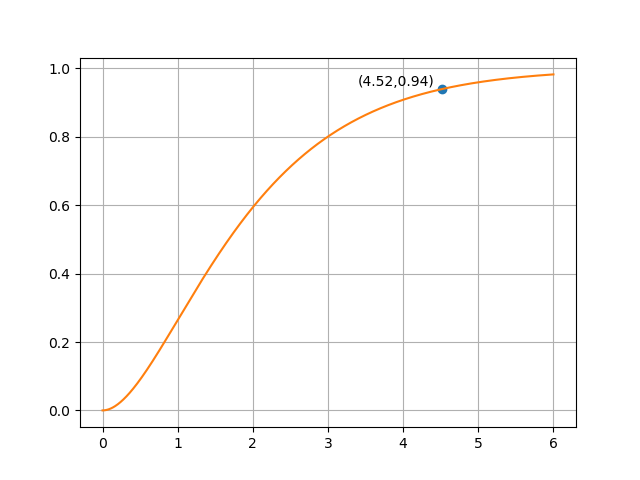
\includegraphics[scale=0.65]{plot.png}
\end{frame}    
\begin{frame}{}
  \centering \Large
  \emph{THANK YOU}
\end{frame}
\end{document}